\documentclass[12pt]{article}
%%%%%%%%%%%%%%%%%%%%%%%%%%%%%%%%%%%%%%%%%%%%%%%%%%%%%%%%%%%%%%%%%%%%%%%%%%%%%%%%%%%%%%%%%%%%%%%%%%%%%%%%%%%%%%%%%%%%%%%%%%%%%%%%%%%%%%%%%%%%%%%%%%%%%%%%%%%%%%%%%%%%%%%%%%%%%%%%%%%%%%%%%%%%%%%%%%%%%%%%%%%%%%%%%%%%%%%%%%%%%%%%%%%%%%%%%%%%%%%%%%%%%%%%%%%%
\usepackage{setspace}
\usepackage{xcolor}
\usepackage{amssymb}
\usepackage{amsmath}
\usepackage{amsfonts}
\usepackage{titlesec}
\usepackage[margin=1.5in]{geometry}
\usepackage{graphicx}
\usepackage[hidelinks]{hyperref}
\usepackage{etoolbox}
\usepackage{xr}
\usepackage{natbib}
\usepackage{lmodern}
\usepackage{standalone}
\usepackage{multirow}
\usepackage{graphicx}
\usepackage{caption,subcaption}
\usepackage{booktabs}
\usepackage{pdflscape}
\setcounter{MaxMatrixCols}{10}
\begin{document}

%\begin{itemize}
%  \item Figure
%\end{itemize}

    \begin{table}
      \caption{Recall rates for E-U-E spells}
      \begin{center}
\begin{tabular}{l|cc}
  \hline \hline
   & \multicolumn{2}{c}{\textit{From}:} \\[0.35em]
                                     &\multicolumn{1}{c}{Temporary} & \multicolumn{1}{c}{Permanent} \\
   \textit{Panel:}                                  
                                     &\multicolumn{1}{c}{layoff} & 
                                     \multicolumn{1}{c}{separation} 
                                     \\[0.35em]
                                     \hline \\[-1em]
  All  & 0.763 & 0.064 \\[.35em]
  1996 & 0.740 & 0.063 \\[.35em]
  2001 & 0.754 & 0.068 \\[.35em]
  2004 & 0.766 & 0.080 \\[.35em]
  2008 & 0.782 & 0.047 \\[.35em]
               \hline
\end{tabular}
    \subcaption*{\small \textit{Note:} [Subcaption TBW]}
      \end{center}
    \end{table}

  \begin{figure}
    \caption{U-to-E Hazards: Recall and New Job-Finding\label{fig:UE}}
  \centerline{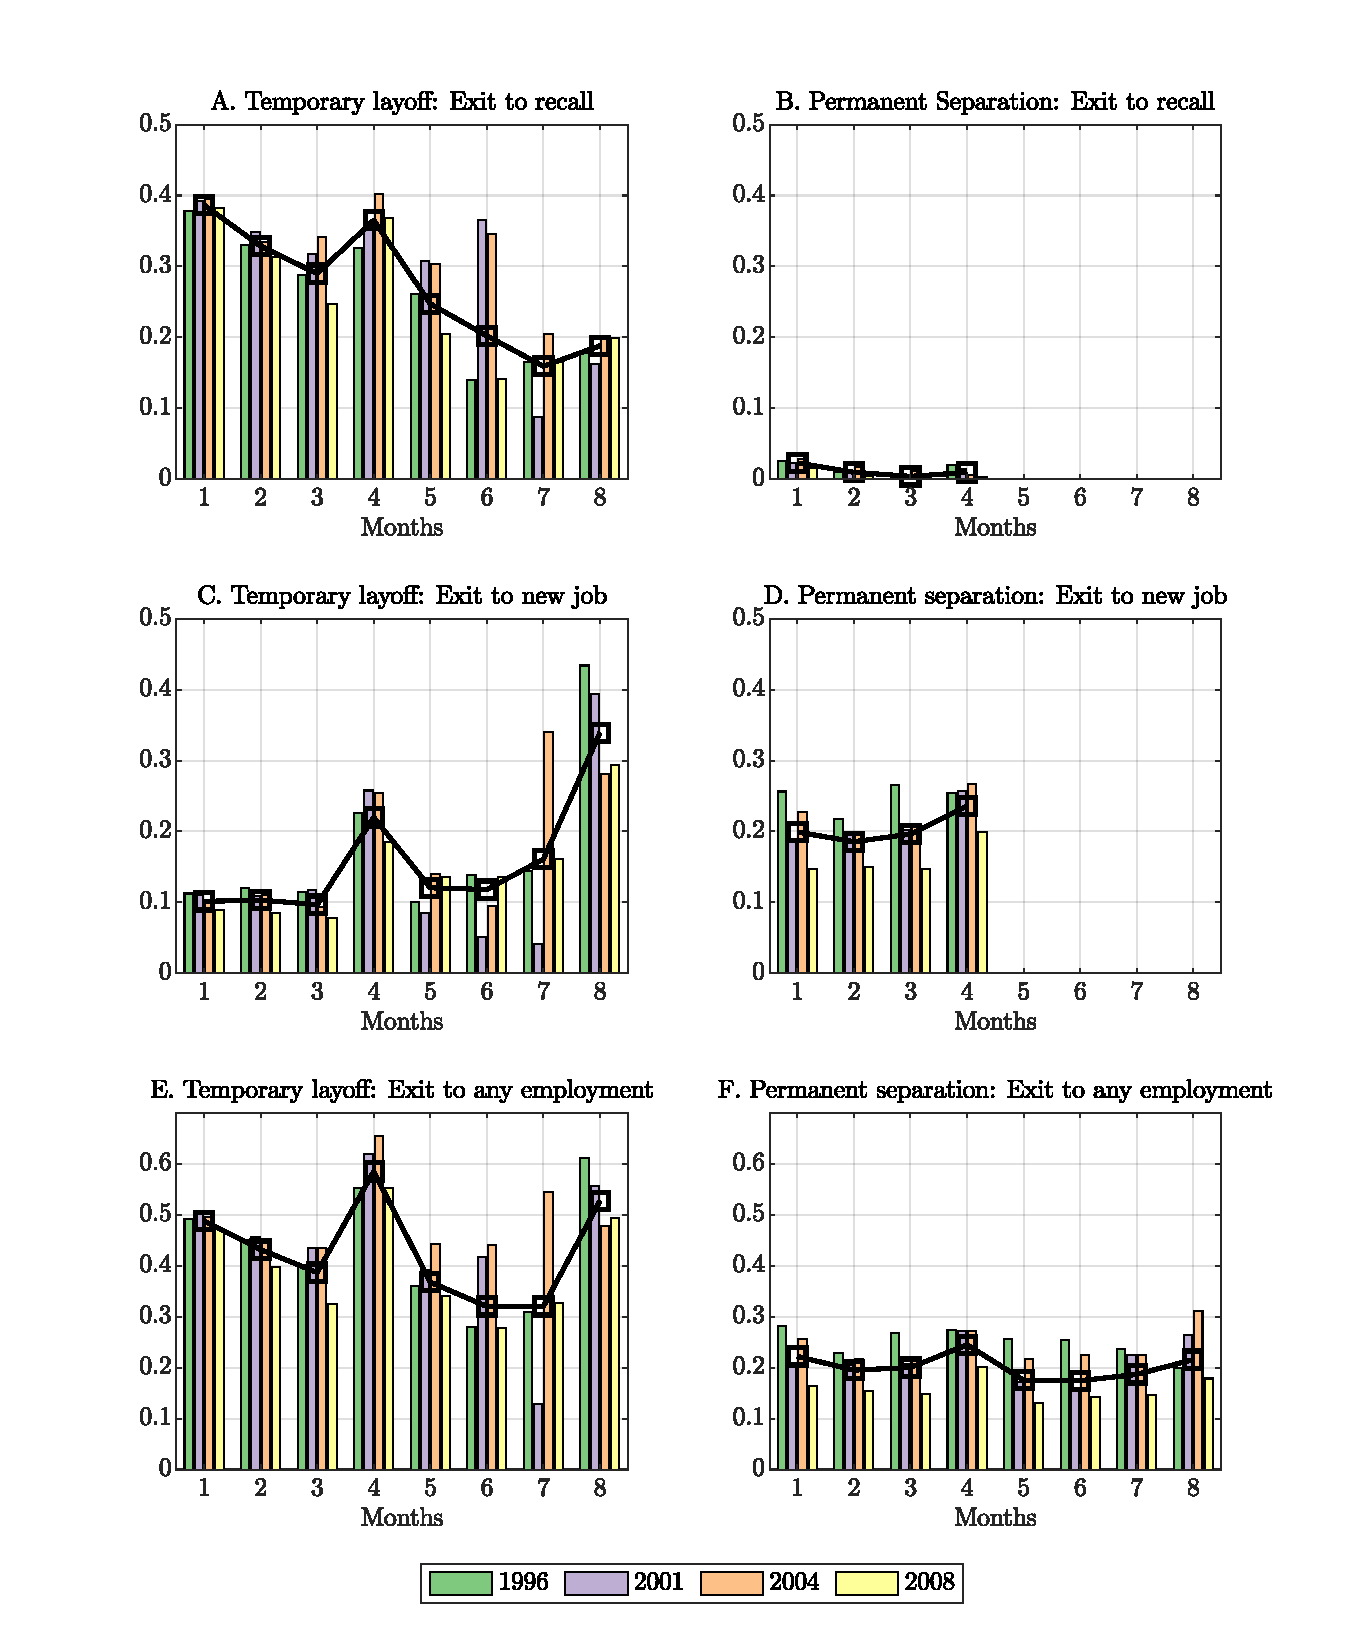
\includegraphics[width=1.00\linewidth]{./../figures/all}}
    \subcaption*{\small \textit{Note:} [Subcaption TBW]}
  \end{figure}

  \begin{figure}
  \caption{SIPP interview structure}
    \begin{center}
      \includegraphics[width=\linewidth]{sipp_waves}
    \end{center}
  \end{figure}

    \begin{table}
      \caption{First reference month of unemployment spell}
      \begin{center}
  \begin{tabular}{l|cccc}
    & \multicolumn{1}{c}{1$^\text{st}$ ref.}
    & \multicolumn{1}{c}{2$^\text{nd}$ ref.}
    & \multicolumn{1}{c}{3$^\text{rd}$ ref.}
    & \multicolumn{1}{c}{4$^\text{th}$ ref.} \\
    & \multicolumn{1}{c}{month}
    & \multicolumn{1}{c}{month}
    & \multicolumn{1}{c}{month}
    & \multicolumn{1}{c}{month} \\ \hline \\[-1em]
    Permanent separations & 0.387 &  0.205 &  
    0.202 &   0.207 \\[.35em]
    Temporary layoffs     & 0.328 &  0.210 &  0.233 &   0.230 \\[.35em]
    \hline
  \end{tabular}
    \subcaption*{\small \textit{Note:} [Subcaption TBW]}
      \end{center}
    \end{table}

    \begin{table}
      \caption{Final reference month of unemployment spell}
      \begin{center}
  \begin{tabular}{l|cccc}
    & \multicolumn{1}{c}{1$^\text{st}$ ref.}
    & \multicolumn{1}{c}{2$^\text{nd}$ ref.}
    & \multicolumn{1}{c}{3$^\text{rd}$ ref.}
    & \multicolumn{1}{c}{4$^\text{th}$ ref.} \\
    & \multicolumn{1}{c}{month}
    & \multicolumn{1}{c}{month}
    & \multicolumn{1}{c}{month}
    & \multicolumn{1}{c}{month} \\ \hline \\[-1em]
    Permanent separations & 0.203 &  0.209 &  
    0.223 &   0.365 \\[.35em]
    Temporary layoffs     & 0.137 &  0.190 &  
    0.236 &   0.437 \\[.35em]
    \hline
  \end{tabular}
    \subcaption*{\small \textit{Note:} [Subcaption TBW]}
      \end{center}
    \end{table}


  \begin{landscape}
    \begin{figure}
    \caption{U-to-E Hazards by Reference Month at Start of Spell: 
    Temporary Layoffs\label{fig:UEtl}}
    \centerline{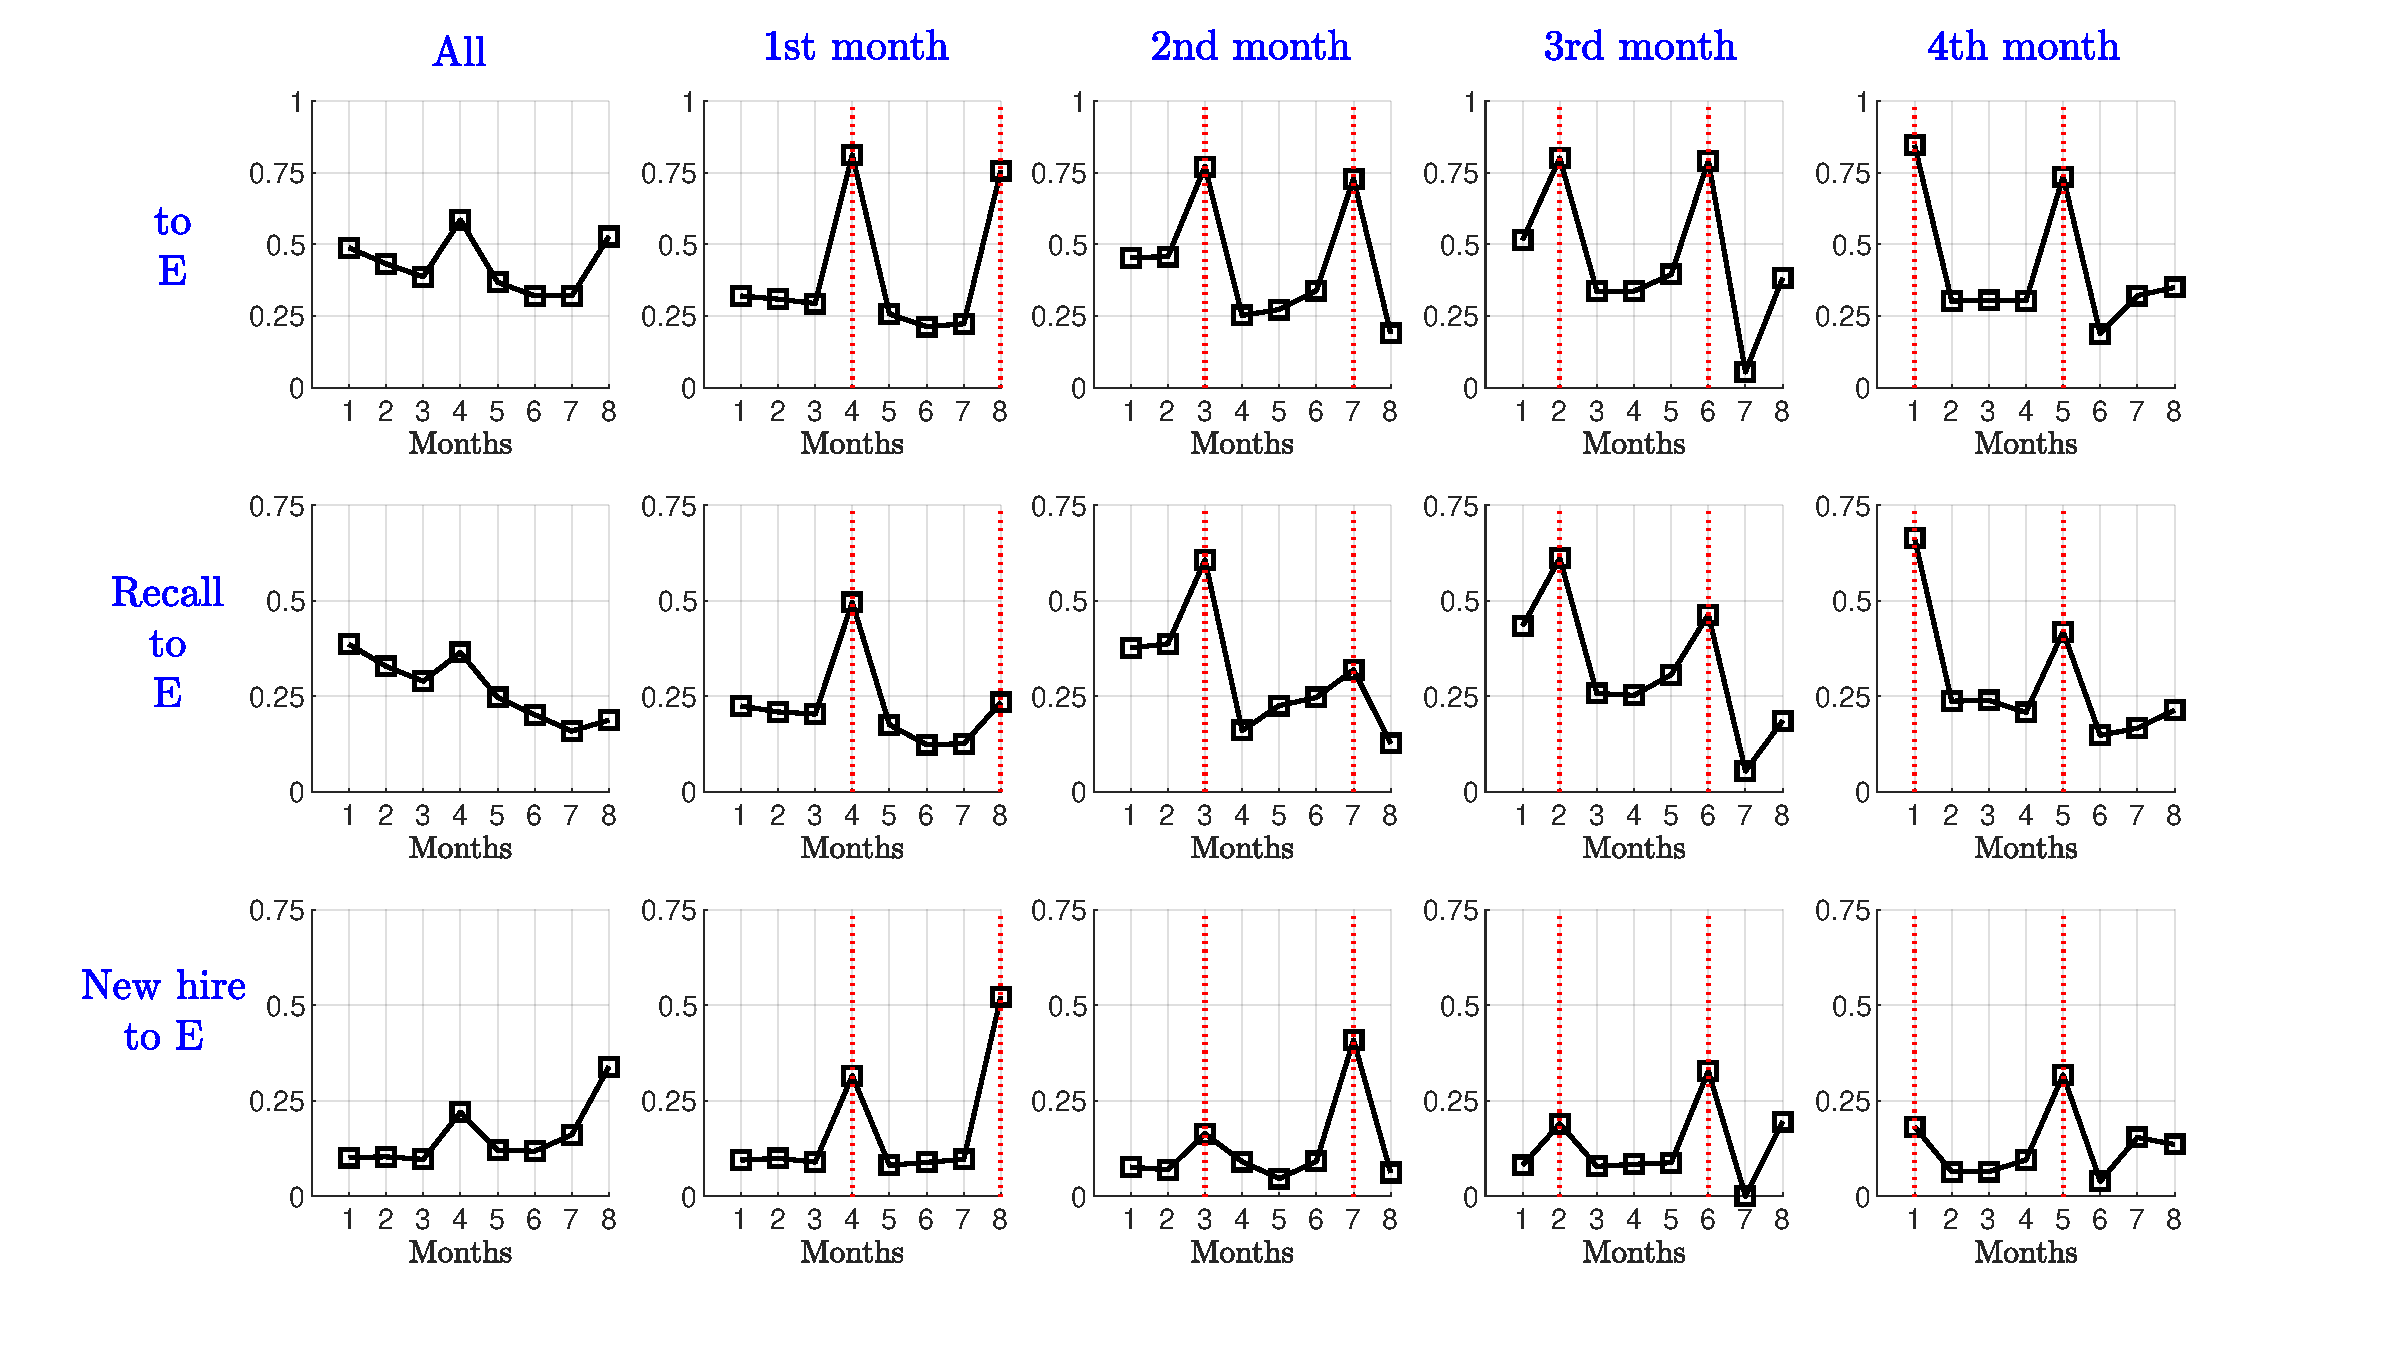
\includegraphics[width=1.00\linewidth]{./../figures/TL}}
    \subcaption*{\small \textit{Note:} [Subcaption TBW]}
    \end{figure}

  \begin{figure}
  \caption{U-to-E Hazards by Reference Month at Start of Spell: 
  Permanent Separations\label{fig:UEtl}}
  \centerline{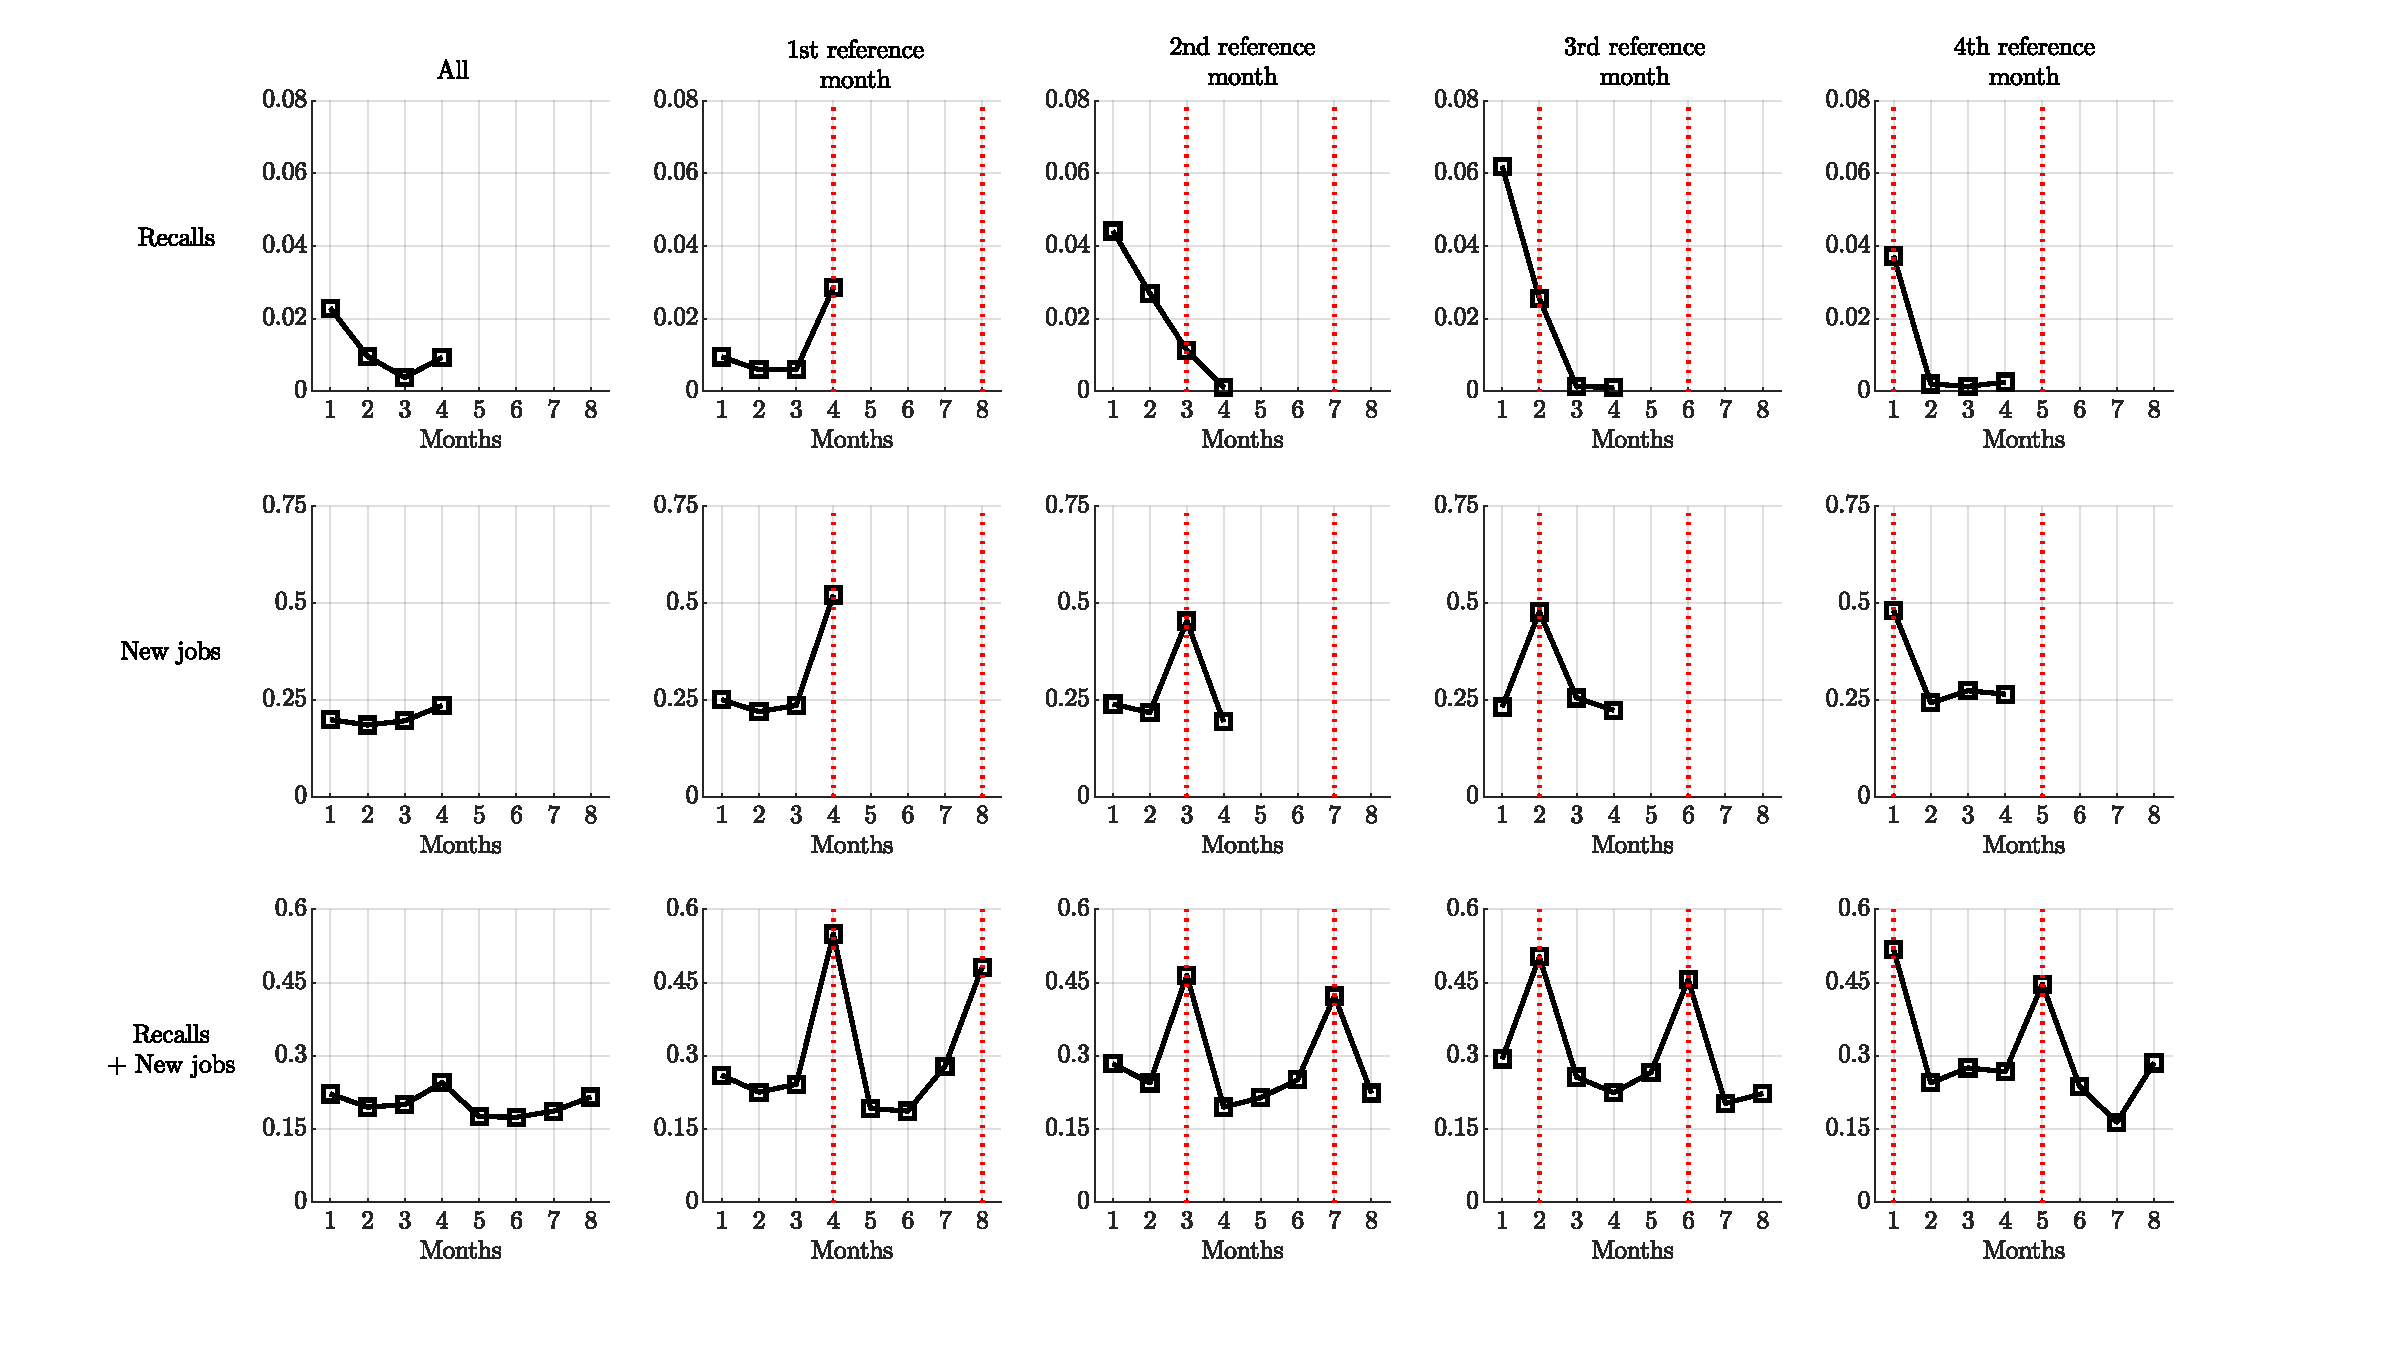
\includegraphics[width=1.00\linewidth]{./../figures/PS}}
    \subcaption*{\small \textit{Note:} [Subcaption TBW]}
  \end{figure}
  \end{landscape}

\end{document}
